\section{Контейнеры компоновки}

\graphicspath{{parts/guides/2_managers/images/}}

\subsection{Общая информация о компоновке} \title{panel_definition}

Компоновка (layout) представляет собой процесс размещения элементов внутри контейнера. С помощью неё в WPF осуществляется процесс позиционирования элементов для реализация адаптивной верстки — подход в верстке, при котором элементы приспосабливаются к изменениям размеров контейнера, на котором они расположены.

В WPF компоновка осуществляется при помощи специальных контейнеров

\mintinline{xml}{Grid}, \mintinline{xml}{UniformGrid}, \mintinline{xml}{StackPanel}, \mintinline{xml}{WrapPanel}, \mintinline{xml}{DockPanel} и \mintinline{xml}{Canvas}.

Различные контейнеры могут содержать внутри себя другие контейнеры. Кроме данных контейнеров существует еще ряд элементов, такие как \mintinline{xml}{TabPanel}, которые могут включать другие элементы и даже контейнеры компоновки, однако на саму компоновку не столь влияют в отличие от перечисленных выше.

Каждый из контейнеров наследуется от абстрактного класса \mintinline{csharp}{Panel}, который в свою очередь наследуется от класса \mintinline{csharp}{FrameworkElement}.

При компоновке элементов нежелательно вручную указывать их точные размеры и расположение элементов, так как определение этих параметров задача контейнера.

Процесс компоновки проходит два этапа: измерение (measure) и расстановка (arrange). На этапе измерения контейнер производит измерение предпочтительного для дочерних элементов места. Однако не всегда имеется достаточно места, чтобы расставить все элементы по их предпочтительным размерам, поэтому их размеры приходится усекать. Затем происходит этап непосредственной расстановки дочерних элементов внутри контейнера.

\subsection{\mintinline{xml}{Grid}} \label{Grid_defenition}

\mintinline{xml}{Grid} - контейнер, определяющий адаптивную сетку, которая состоит из строк, определяемых через \mintinline{xml}{RowDefinitions}, и столбцов, определяемых через \mintinline{xml}{ColumnDefinitions}. Пример использование такого контейнера

\begin{minted}{xml}
<Grid>
    <Grid.RowDefinitions>
        <RowDefinition />
        <RowDefinition />
        <RowDefinition />
    </Grid.RowDefinitions>
    <Grid.ColumnDefinitions>
        <ColumnDefinition />
        <ColumnDefinition />
        <ColumnDefinition />
    </Grid.ColumnDefinitions>
    
    <!-- Тут может находиться какой-то код -->
</Grid>
\end{minted}

В данном случае у нас определено 3 строки и 3 столбца.

Чтобы задать позицию элемента управления с привязкой к определенной ячейке \mintinline{xml}{Grid}, в разметке элемента нужно прописать значения свойств \mintinline{xml}{Grid.Column} и \mintinline{xml}{Grid.Row}, тем самым указывая, в каком столбце и строке будет находиться элемент. Кроме того, если мы хотим растянуть элемент управления на несколько строк или столбцов, то можно указать свойства \mintinline{xml}{Grid.ColumnSpan} и \mintinline{xml}{Grid.RowSpan}, как в следующем примере:

\begin{minted}{xml}
<Grid ShowGridLines="True">
    <Grid.RowDefinitions>
        <RowDefinition></RowDefinition>
        <RowDefinition></RowDefinition>
        <RowDefinition></RowDefinition>
    </Grid.RowDefinitions>
    <Grid.ColumnDefinitions>
        <ColumnDefinition></ColumnDefinition>
        <ColumnDefinition></ColumnDefinition>
        <ColumnDefinition></ColumnDefinition>
    </Grid.ColumnDefinitions>
    <TextBlock Grid.Column="0" Grid.Row="0" Text="Столбец 0 Строка 0" />
    <TextBlock Grid.Column="0" Grid.Row="1" Grid.ColumnSpan="3" 
        Text="Объединение трех столбцов, строка 1" 
        VerticalAlignment="Center" 
        HorizontalAlignment="Center" 
        FontSize="40" 
    />
    <TextBlock Grid.Column="2" Grid.Row="2" Text="Строка 2 Столбец 2" />
</Grid>
\end{minted}

В результате получим:

\begin{figure}[H]
\centering
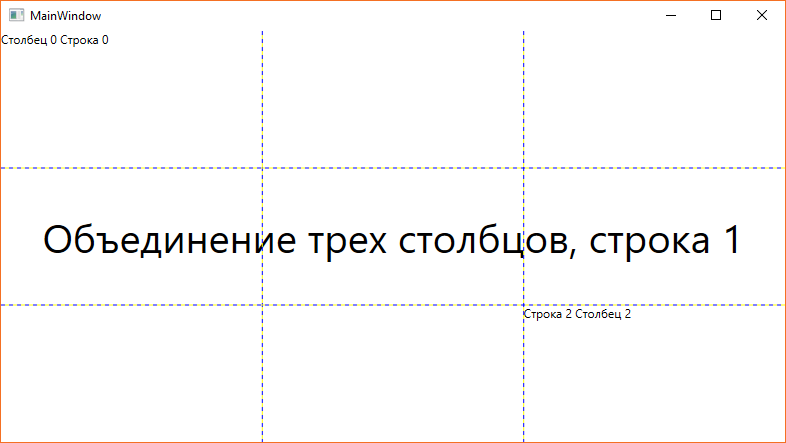
\includegraphics[width=1\textwidth]{manager_grid.png}
\end{figure}


Свойство \mintinline{xml}{ShowGridLines="True"} у элемента \mintinline{xml}{Grid} задает видимость сетки.

При определении строк и столбцов можно указать их размеры. Делается это тремя способами

\begin{description}[style=nextline]
\item [Автоматические размеры] Здесь столбец или строка занимает столько места, сколько им нужно

\begin{minted}{xml}
<ColumnDefinition Width="Auto" />
<RowDefinition Height="Auto" />
\end{minted}

\item [Абсолютные размеры] В данном случае высота и ширина указываются в единицах, независимых от устройства:

\begin{minted}{xml}
<ColumnDefinition Width="150" />
<RowDefinition Height="150" />
\end{minted}

Также абсолютные размеры можно задать в пикселях (\mintinline{xml}{px}), дюймах (\mintinline{xml}{in}), сантиметрах (\mintinline{xml}{cm}) или точках (\mintinline{xml}{pt}):

\begin{minted}{xml}
<ColumnDefinition Width="1 in" />
<RowDefinition Height="10 px" />
\end{minted}

\item [Пропорциональные размеры] Например, ниже задаются два столбца, второй из которых имеет ширину в четверть от ширины первого:

\begin{minted}{xml}
<ColumnDefinition Width="*" />
<ColumnDefinition Width="0.25*" />
\end{minted}

\end{description}


Если строка или столбец имеет высоту, равную \mintinline{xml}{*}, то данная строка или столбец будет занимать все оставшееся место. Если есть несколько сток или столбцов, высота которых равна \mintinline{xml}{*}, то все доступное место делится поровну между всеми такими сроками и столбцами. Также возможно использование коэффициентов (например \mintinline{xml}{0.25*}). При этом все коэффициенты складываются (\mintinline{xml}{коэффициент * аналогичен 1*}) и затем все пространство делится на сумму коэффициентов.

Например, если 3 столбца:

\begin{minted}{xml}
<ColumnDefinition Width="*" />
<ColumnDefinition Width="0.5*" />
<ColumnDefinition Width="1.5*" />
\end{minted}


В этом случае сумма коэффициентов равна \mintinline{csharp}{1* + 0.5* + 1.5* = 3*}. Если сетка имеет ширину 300 единиц, то коэффициент \mintinline{xml}{1*} будет соответствовать пространству \mintinline{csharp}{300 / 3 = 100} единиц. Поэтому первый столбец будет иметь ширину в \mintinline{csharp}{100} единиц, второй \mintinline{csharp}{100 * 0.5 = 50} единиц, а третий \mintinline{csharp}{100 * 1.5 = 150} единиц.

Можно комбинировать все типы размеров. В этом случае от ширины/высоты сетки отнимается ширина/высота столбцов/строк с абсолютными или автоматическими размерами, и затем оставшееся место распределяется между столбцами/строками с пропорциональными размерами.

\subsection{\mintinline{xml}{UniformGrid}}

Аналогичен контейнеру \mintinline{xml}{Grid} контейнер \mintinline{xml}{UniformGrid}, только в этом случае все столбцы и строки одинакового размера и используется упрощенный синтаксис для их определения

\begin{minted}{xml}
<UniformGrid Rows="2" Columns="2">
    <Button Content="Left Top" />
    <Button Content="Right Top" />
    <Button Content="Left Bottom" />
    <Button Content="Right Bottom" />
</UniformGrid>
\end{minted}

\subsection{\mintinline{xml}{StackPanel}}

Это более простой элемент компоновки. Он располагает все элементы в ряд либо по горизонтали, либо по вертикали в зависимости от ориентации.

В данном случае для свойства \mintinline{xml}{Orientation} по умолчанию используется значение \mintinline{xml}{Vertical}, то есть \mintinline{xml}{StackPanel} создает вертикальный ряд, в который помещает все вложенные элементы сверху вниз. Мы также можем задать горизонтальный стек. Для этого нам надо указать свойство \mintinline{xml}{Orientation="Horizontal"}:

\begin{minted}{xml}
<Window x:Class="StackPanelTest.MainWindow"
        xmlns="http://schemas.microsoft.com/winfx/2006/xaml/presentation"
        xmlns:x="http://schemas.microsoft.com/winfx/2006/xaml"
        xmlns:d="http://schemas.microsoft.com/expression/blend/2008"
        xmlns:mc="http://schemas.openxmlformats.org/markup-compatibility/2006"
        xmlns:local="clr-namespace:StackPanelTest"
        mc:Ignorable="d"
        Title="MainWindow" Height="450" Width="800">

    <Grid>
        <Grid.RowDefinitions>
            <RowDefinition Height="Auto" />
            <RowDefinition Height="*" />
        </Grid.RowDefinitions>
        
        <StackPanel Grid.Row="0" Margin="10">
            <Button Background="White" Content="1" />
            <Button Background="Blue" Content="2" />
            <Button Background="Red" Content="3" />
        </StackPanel>

        <StackPanel Grid.Row="1" Margin="10" Orientation="Horizontal">
            <Button Background="White" MinWidth="30" Content="4" />
            <Button Background="Blue" MinWidth="30" Content="5" />
            <Button Background="Red" MinWidth="30" Content="6" />
        </StackPanel>
    </Grid>
</Window>
\end{minted}

\newpage
Результат:

\begin{figure}[H]
\centering
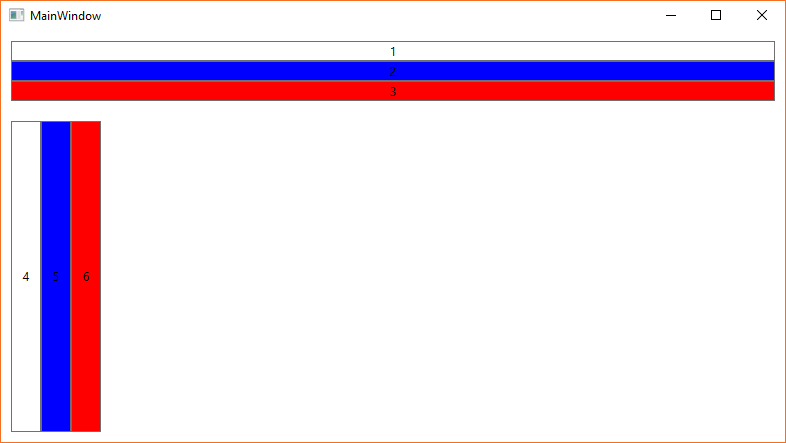
\includegraphics[width=1\textwidth]{manager_stackpanel.png}
\end{figure}

При горизонтальной ориентации все вложенные элементы располагаются слева направо. Если мы хотим, чтобы наполнение стека начиналось справа налево, то нам надо задать свойство \mintinline{xml}{FlowDirection}.

\begin{minted}{xml}
<StackPanel Orientation="Horizontal" FlowDirection="RightToLeft">
\end{minted}

По умолчанию это свойство имеет значение \mintinline{xml}{LeftToRight} — то есть слева направо.

\subsection{\mintinline{xml}{DockPanel}}

Этот контейнер прижимает свое содержимое к определенной стороне внешнего контейнера. Для этого у вложенных элементов надо установить сторону, к которой они будут прижиматься с помощью свойства \mintinline{xml}{DockPanel.Dock}. Например:

В итоге получаем массив кнопок, каждая из которых прижимается к определенной стороне элемента \mintinline{xml}{DockPanel}:

\newpage

\begin{minted}{xml}
<Window x:Class="DockPanelTest.MainWindow"
        xmlns="http://schemas.microsoft.com/winfx/2006/xaml/presentation"
        xmlns:x="http://schemas.microsoft.com/winfx/2006/xaml"
        xmlns:d="http://schemas.microsoft.com/expression/blend/2008"
        xmlns:mc="http://schemas.openxmlformats.org/markup-compatibility/2006"
        xmlns:local="clr-namespace:DockPanelTest"
        mc:Ignorable="d"
        Title="MainWindow" Height="450" Width="800">

    <Grid>
        <DockPanel LastChildFill="True">
            <Button 
                DockPanel.Dock="Top" 
                Background="Orange" 
                Content="Dock Top 1" />
            <Button 
                DockPanel.Dock="Top" 
                Background="Orange" 
                Content="Dock Top 2" />
            <Button 
                DockPanel.Dock="Bottom" 
                Background="IndianRed" 
                Content="Dock Bottom" />
            <Button 
                DockPanel.Dock="Left" 
                Background="Aquamarine" 
                Content="Dock Left 1" />
            <Button 
                DockPanel.Dock="Left" 
                Background="Aquamarine" 
                Content="Dock Left 2" />
            <Button 
                DockPanel.Dock="Right" 
                Background="Azure" 
                Content="Dock Right" />
            <Button 
                Background="DodgerBlue" 
                Content="Dock Center (last)" />
        </DockPanel>
    </Grid>
</Window>
\end{minted}

\newpage
Результат:

\begin{figure}[H]
\centering
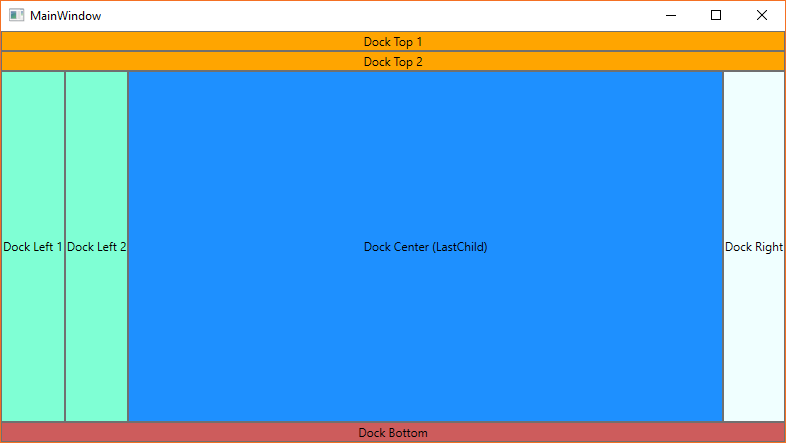
\includegraphics[width=1\textwidth]{manager_dockpanel.png}
\end{figure}


Причем у последней кнопки мы можем не устанавливать свойство \mintinline{xml}{DockPanel.Dock}. Она уже заполняет все оставшееся пространство. Такой эффект получается благодаря установке у \mintinline{xml}{DockPanel} свойства \mintinline{xml}{LastChildFill="True"}, которое означает, что последний элемент заполняет все оставшееся место. Если у этого свойства поменять \mintinline{xml}{True} на \mintinline{xml}{False}, то кнопка прижмется к левой стороне, заполнив только о место, которое ей необходимо.

Контейнер \mintinline{xml}{DockPanel} особенно удобно использовать для создания стандартных интерфейсов, где верхнюю и левую часть могут занимать какие-либо меню, нижнюю — строка состояния, правую — какая-то дополнительная информация, а в центре будет находиться основное содержание.

\subsection{\mintinline{xml}{WrapPanel}}

Эта панель, подобно \mintinline{xml}{StackPanel}, располагает все элементы в одной строке или колонке в зависимости от того, какое значение имеет свойство \mintinline{xml}{Orientation} — \mintinline{xml}{Horizontal} или \mintinline{xml}{Vertical}. Главное отличие от \mintinline{xml}{StackPanel}, если элементы не помещаются в строке или столбце, создаются новые столбец или строка для не поместившихся элементов.

В горизонтальном стеке те элементы, у которых явным образом не установлена высота, будут автоматически принимать высоту самого большого элемента из стека.

В вертикальном стеке элементы, у которых явным образом не указана ширина, автоматически принимают ширину самого широкого элемента.

Мы также можем установить для всех вложенных элементов какую-нибудь определенную ширину (с помощью свойства \mintinline{xml}{ItemWidth}) или высоту (свойство \mintinline{xml}{ItemHeight}).

Расммотрим пример использования \mintinline{xml}{WrapPanel}

\begin{minted}{xml}
<Window x:Class="WrapPanelTest.MainWindow"
        xmlns="http://schemas.microsoft.com/winfx/2006/xaml/presentation"
        xmlns:x="http://schemas.microsoft.com/winfx/2006/xaml"
        xmlns:d="http://schemas.microsoft.com/expression/blend/2008"
        xmlns:mc="http://schemas.openxmlformats.org/markup-compatibility/2006"
        xmlns:local="clr-namespace:WrapPanelTest"
        mc:Ignorable="d"
        Title="MainWindow" Height="450" Width="400">

    <Grid>
        <WrapPanel>
            <Button Background="AliceBlue" Content="1" Width="200" />
            <Button Background="Blue" Content="2" Width="100" />
            <Button Background="Aquamarine" Content="3" Width="100" Height="30" />
            <Button Background="DarkGreen" Content="4" Height="20" />
            <Button Background="LightGreen" Content="5" Width="200" />
            <Button Background="RosyBrown" Content="6" Width="80" />
            <Button Background="GhostWhite" Content="7" />
        </WrapPanel>
    </Grid>
</Window>
\end{minted}

Результат:
\begin{figure}[H]
\centering
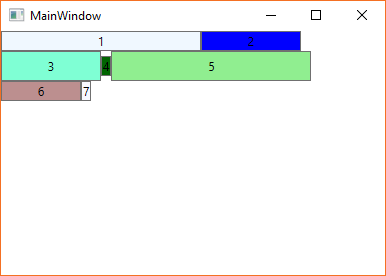
\includegraphics[width=0.5\textwidth]{manager_wrappanel.png}
\end{figure}

\subsection{\mintinline{xml}{Canvas}}

Контейнер \mintinline{xml}{Canvas} является наиболее простым контейнером. Для размещения на нем необходимо указать для элементов точные координаты относительно сторон \mintinline{xml}{Canvas}. Для установки координат элементов используются свойства \mintinline{xml}{Canvas.Left}, \mintinline{xml}{Canvas.Right}, \mintinline{xml}{Canvas.Bottom}, \mintinline{xml}{Canvas.Top}. Например, свойство \mintinline{xml}{Canvas.Left} указывает, на сколько единиц от левой стороны контейнера будет находиться элемент, а свойство \mintinline{xml}{Canvas.Top} сколько единиц ниже верхней границы контейнера находится элемент.

При этом в качестве единиц используются не пиксели, а независимые от устройства единицы, которые помогают эффективно управлять масштабированием элементов. Каждая такая единица равна \mintinline{xml}{1/96} дюйма, и при стандартной установке в \mintinline{xml}{96 dpi} эта независимая от устройства единица будет равна физическому пикселю. В тоже время при работе на других мониторах или при других установленных размеры, установленные в приложении, будут эффективно масштабироваться. Например, при разрешении в \mintinline{xml}{120 dpi} одна условная единица будет равна 1.25 пикселя.

Если элемент не использует свойства \mintinline{xml}{Canvas.Top} и другие, то по умолчанию свойства \mintinline{xml}{Canvas.Left} и \mintinline{xml}{Canvas.Top} будут равны нулю, то есть он будет находиться в верхнем левом углу.

Также надо учитывать, что нельзя одновременно задавать \mintinline{xml}{Canvas.Left} и \mintinline{xml}{Canvas.Right} или \mintinline{xml}{Canvas.Bottom} и \mintinline{xml}{Canvas.Top}. Если подобное произойдет, то последнее заданное свойство не будет учитываться. 

Пример использования:

\begin{minted}{xml}
<Window x:Class="CanvasTest.MainWindow"
        xmlns="http://schemas.microsoft.com/winfx/2006/xaml/presentation"
        xmlns:x="http://schemas.microsoft.com/winfx/2006/xaml"
        xmlns:d="http://schemas.microsoft.com/expression/blend/2008"
        xmlns:mc="http://schemas.openxmlformats.org/markup-compatibility/2006"
        xmlns:local="clr-namespace:CanvasTest"
        mc:Ignorable="d"
        Title="MainWindow" Height="450" Width="600">

    <Grid>
        <Canvas Background="SteelBlue">
            <Rectangle Fill="Orange" 
                Width="150" Height="50" Canvas.Top="20" Canvas.Left="40" />
                
            <Ellipse Fill="Red" 
                Width="150" Height="150" Canvas.Top="60" Canvas.Left="240" />
                
            <Button Content="Button" 
                Width="150" Height="50" Canvas.Bottom="260" Canvas.Right="220" />
        </Canvas>
    </Grid>
</Window>
\end{minted}

\newpage
Результат:
\begin{figure}[H]
\centering
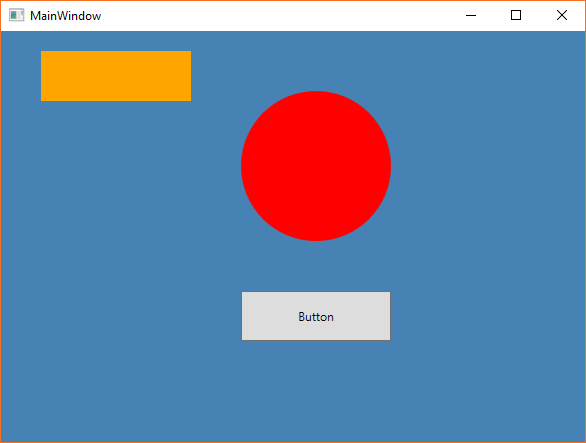
\includegraphics[width=0.8\textwidth]{manager_canvas.png}
\end{figure}